\documentclass [xcolor=svgnames, t] {beamer} 
\usepackage[utf8]{inputenc}
\usepackage{booktabs, comment} 
\usepackage[absolute, overlay]{textpos} 
\usepackage{pgfpages}
\usepackage[font=footnotesize]{caption}
\useoutertheme{infolines} 



%\definecolor{brownbrown}{RGB}{56, 28, 0}
%\definecolor{brownred}{RGB}{228, 0, 43}

%\setbeamercolor{title in head/foot}{bg=brownred, fg=brownbrown}
%\setbeamercolor{author in head/foot}{bg=myuniversity}
\setbeamertemplate{page number in head/foot}{}
\usepackage{csquotes}


\usepackage{amsmath}
\usepackage[makeroom]{cancel}


\usepackage{textpos}

\usepackage{tikz}
\usetikzlibrary{shapes.geometric}
\usetikzlibrary{positioning}
%\tikzset{
%  every overlay node/.style={
%    draw=black,fill=white,rounded corners,anchor=south west,
%  },
%}
% Usage:
% \tikzoverlay at (-1cm,-5cm) {content};
% or
% \tikzoverlay[text width=5cm] at (-1cm,-5cm) {content};
%\def\tikzoverlay{%
%   \tikz[baseline,overlay]\node[every overlay node]
%}%
\tikzset{
  every overlay node/.style={
    anchor=north west,
  },
}
\def\tikzoverlay{%
   \tikz[baseline,overlay]\node[every overlay node]
}%


\newenvironment{smallgreentext}{\scriptsize\color{green}}{\par}
\newenvironment{smallbluetext}{\scriptsize\color{blue}}{\par}
\def\checkmark{\tikz\fill[scale=0.4](0,.35) -- (.25,0) -- (1,.7) -- (.25,.15) -- cycle;}
\usetheme{Madrid}
%\definecolor{myuniversity}{RGB}{56, 28, 0}
%\usecolortheme[named=myuniversity]{structure}

\title[Estructura del documento]{Clase No.03: Estructura del documento}
\subtitle{Revisi\'on de la plantilla del documento}
\institute[]{Departamento de Ingenier\'ia Civil y Agr\'icola\\ Facultad de Ingenier\'ia  \\Universidad Nacional de Colombia - Sede Bogot\'a}
\titlegraphic{\includegraphics[height=2.0cm]{escudoUnal.png}}
\author[LAM]{Luis Alejandro Morales \\ \href{https://lamhydro.github.io}{https://lamhydro.github.io}}
%\date{\today}
\date{}


\addtobeamertemplate{navigation symbols}{}{%
    \usebeamerfont{footline}%
    \usebeamercolor[fg]{footline}%
    \hspace{1em}%
    \insertframenumber/\inserttotalframenumber
}

\begin{document}
\begin{frame}
\maketitle
\end{frame}


%%%%%%%%%%%%%%%%%%%%%%%%%%%%
\logo{\vspace{-0.2cm}\includegraphics[height=0.8cm]{escudoUnal.png}~%
}
%%%%%%%%%%%%%%%%%%%%%%%%%%



\begin{frame}
\frametitle{Table of Contents}
\tableofcontents
\end{frame}


%%%%%%%%
\section{Normatividad}
\begin{frame}{Normatividad}
\vspace{-0.3cm}
\centering
\includegraphics[width=\textwidth]{norm}
\small{Articulo 20: \emph{Contenido del Documento de Proyecto de T\'esis de Maestr\'ia}}
\centering
\includegraphics[width=\textwidth]{norm1}
\end{frame}
\begin{frame}{Normatividad}
\centering
\includegraphics[width=\textwidth]{norm2}
\end{frame}

%%%%%%%%
\section{Indice general de un documento de t\'esis or proyecto}

\begin{frame}{Indice del documento}
\begin{columns}[T]
\column{0.3\textwidth}
El indice de un trabajo final de maestr\'ia, es la \alert{carta de navegación del proyecto}. Esta puede cambiar y se puede modificar de acuerdo con las necesidades que surjan en la realización del proyecto. 
\column{0.7\textwidth}
\centering
\includegraphics[width=\textwidth]{thesisIndx}
\end{columns}
\tikzoverlay[text width=3cm] at (5.1cm,5.2cm) {
\begin{smallgreentext}
(\href{https://bibliotecas.unal.edu.co/servicios/servicios-en-linea/entrega-de-tesis-y-publicaciones-en-linea}{https://bibliotecas.unal.edu.co/servicios/servicios-en-linea/entrega-de-tesis-y-publicaciones-en-linea})
\end{smallgreentext}
};
\end{frame}


\begin{frame}{Indice del documento}
Estructura general de un documento de proyecto de tesis:
\begin{columns}[T]
\column{0.2\textwidth}
\scriptsize{
\begin{itemize}
\item T\'itulo
\item Resumen
\item Introducci\'on
\item Metodolog\'ia 
\item Resultados
\item Discusión
\item Conclusiones
\item Bibliograf\'ia
\item Anexos
\end{itemize}
}
\column{0.4\textwidth}
\centering
\includegraphics[width=\textwidth]{idx1}
\column{0.4\textwidth}
\centering
\includegraphics[width=\textwidth]{idx2}
\end{columns}
\tikzoverlay[text width=3cm] at (3cm,0cm) {
\begin{smallgreentext}
(\href{https://repositorio.unal.edu.co/handle/unal/69784}{https://repositorio.unal.edu.co/handle/unal/69784})
\end{smallgreentext}
};
\end{frame}


\begin{frame}{Creaci\'on de secciones}
\begin{itemize}
\item Muestran la estrategia o propósito del documento.
\item Deben revelar la organizaci\'on del documento por si solos.
\item Sirven como breve descanso mental para el lector. 
\item Las secciones sirven como medio para la comprensión del texto. 
\item Piensen sus secciones como tajadas de una torta, deben tener cierto nivel de relaci\'on.
\item Deben seguir una misma estructura gramatical:
\begin{table}
\begin{tabular}{c  c }
\textbf{Frases sustantivas} & \textbf{Frases en participio}\\
Caso de estudio & Conocimiento del la zona de estudio \\
Modelo de la cuenca & Modelaci\'on de cuenca \\
Datos adquiridos & Adquicisi\'on de datos 
\end{tabular}
\end{table}
\end{itemize}
\tikzoverlay[text width=10.5cm] at (0.6cm,0.3cm) {
\centering
\begin{smallbluetext}
\Large El propósito no es siempre que el documento sea leído completamente, si no es informar y persuadir al lector de la manera m\'as eficiente. 
\end{smallbluetext} 
};
\end{frame}


\begin{frame}{Como crear el indice del documento}
\begin{enumerate}
\item Desarrolle una versi\'on inicial con secciones y subsecciones.
\item Iterar las veces que sea necesario sobre la versi\'on inicial agregando/quitando todas las subsecciones que sean necesarias.
\item Identificar figuras y tablas claves por subsecci\'on.
\item Note que cada subsecci\'on se convierte en el tema para desarrollar un párrafo.
\end{enumerate}
\end{frame}

%%%%%%%%

\section{Estructura del documento}
\begin{frame}{Titulo}
El titulo debe reflejar y ser congruente con el \alert{objetivo principal}. El t\'itulo debe cumplir dos funciones:
\begin{itemize}
\item \alert{Atraer} a otros para leer el documento
\item Proporcionar la \alert{mejor información posible} para, e.j. agilizar la búsqueda
\end{itemize}
\emph{¿Como construir un buen titulo?}
\begin{enumerate}
\item Escoger las \alert{palabras claves} en su proyecto.
\item Ordenar las palabras claves de acuerdo con su \alert{importancia}.
\item Construya el titulo colocando las \alert{palabras} de acuerdo con el \alert{orden de importancia}.
\item Si el titulo es \alert{muy largo}, \alert{borre} las palabras menos importantes. 
\end{enumerate}
\tikzoverlay[text width=12cm] at (1cm,0.5cm) {
\begin{smallgreentext}
The influence of season of calving on the performance of Holstein cows.
\end{smallgreentext}
\begin{smallbluetext}
Holstein cows produce more milk if they calve in spring instead of autumn. \checkmark
\end{smallbluetext} 
};
\end{frame}

\begin{frame}{Resumen}
\tikzoverlay[text width=12.5cm] at (-0.2cm,0.8cm) {
\begin{smallbluetext}
"Please be goog enough to put your conclusions and recomendations on one sheet of paper at the very beginning of your report, so that I can even consider reading it" Winston Churchill
\end{smallbluetext} 
};
\begin{minipage}[t]{1.03\textwidth} 
Es una \alert{mini t\'esis} o trabajo. Generalmente es lo que primero y lo que \alert{m\'as se lee} despu\'es del t\'itulo. Caracter\'isticas del resumen:
\begin{itemize}
\item Debe escribirse en \alert{Espa\~nol} y en \alert{Ingl\'es}.
\item Debe incluir las \alert{palabras claves}.
\item Debe incluir entre \alert{150 y 250 palabras}.
\end{itemize}
Componentes esenciales de un resumen
\begin{enumerate}
\item ¿Cual es la motivaci\'on o justificaci\'on del proyecto? \alert{¿Porqu\'e?}
\item ¿Que metodología, sitio de estudio y datos se usaron en el proyecto? \alert{¿C\'omo?}
\item ¿Que se encontró (resultados) después de desarrollar el proyecto? \alert{Resultados principales}
\item ¿Cual es la conclusi\'on con base en los resultados encontrados?\alert{Conclusión principal}
\end{enumerate}
\end{minipage}
\end{frame}

\begin{frame}{Bad and good abstracs}
\includegraphics[width=0.9\textwidth]{badGood}
\tikzoverlay[text width=1.5cm] at (-0.2cm,6cm) {
\includegraphics[width=\textwidth]{X}
};
\tikzoverlay[text width=1.5cm] at (-0.3cm,2.8cm) {
\includegraphics[width=\textwidth]{chm}
};
\end{frame}

\begin{frame}{Introducci\'on}
\begin{columns}[T]
\column{0.5\textwidth}
\begin{itemize}
\item Definir el alcance de el estudio
\item Definir el problema 
\item Establecer el objetivo
\item Identificar vacíos en el tema
\item Establecer el propósito del experimento
\item Resumir los bases del estudio
\item Establecer la pregunta de investigaci\'on
\item Proveer un contexto del proyecto
\item Explicar la teoría involucrada
\item Presentar una hip\'otesis
\end{itemize}
\column{0.5\textwidth}
\begin{itemize}
\item ¿De que es exactamente el trabajo?
\item ¿Por que el trabajo es importante?
\item ¿Que se necesita para entender el trabajo?
\item ¿Como el trabajo sera presentado?
\end{itemize}
\end{columns}
\end{frame}

\begin{frame}{Introducci\'on}
The topdown approach
\tikzoverlay[text width=1.5cm] at (-4.3cm,-1cm) {
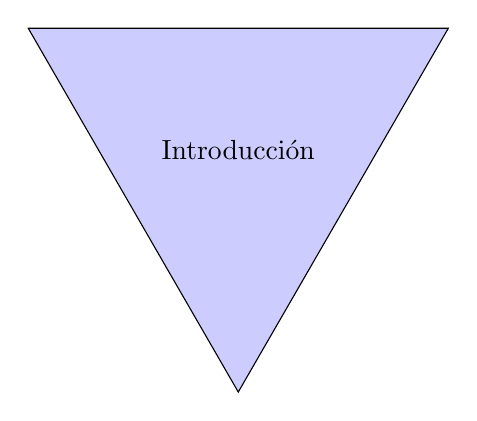
\begin{tikzpicture} 
% \node[regular polygon,regular polygon sides=3, draw, fill=blue!20, shape border rotate=180] at (-4cm,0){Introducci\'on};
 \node[regular polygon,regular polygon sides=3, draw, fill=blue!20, shape border rotate=180] at (current page.center){Introducci\'on};
\end{tikzpicture}
};
\tikzoverlay[text width=4.5cm] at (2.3cm,-1cm) {
\alert{What is the status quo?}
};
\tikzoverlay[text width=4.5cm] at (2.3cm,-3cm) {
\alert{What is wrong with the status quo?}
};
\tikzoverlay[text width=4.5cm] at (2.3cm,-5cm) {
\alert{How does my project/paper go beyond the status quo?}
};
\end{frame}

\begin{frame}{Introducci\'on}
Leer el siguiente \href{https://doi.org/10.1029/2023WR034875}{\alert{paper}} y determine las partes que componen "the topdown approach".
\end{frame}

\begin{frame}{Metodología}

\begin{itemize}
\item Se describe lo que se hizo. 
\item \alert{Relativamente fácil de escribir porque no requiere interpretaciones.}
\item Comúnmente conformada por:
\begin{itemize}
\item Caso de estudio. E.j. Lugar geogr\'afico.
\item Informaci\'on: E.j. Series temporales de precipitación del IDEAM.
\item Métodos anal\'iticos/num\'ericos. E.j. Solución de las ecuaciones de Saint-Venant.
\item Métodos estadístico. E.j. Regresiones multivariadas.
\item Experimentos. En campo o en laboratorio.
\item Diseños de instrumentos.
\end{itemize}
\end{itemize}
\tikzoverlay[text width=8.5cm] at (1.5cm,-0.5cm) {
\centering
\begin{smallbluetext}
\large Un lector debe ser capaz de reproducir lo que se realiz\'o de acuerdo a lo descrito en la metodolog\'ia
\end{smallbluetext} 
};
\end{frame}


\begin{frame}{Metodolog\'ia}
Leer el siguiente \href{https://doi.org/10.1029/2023WR034875}{\alert{paper}} y determine los m\'etodos, zona de estudio e informaci\'on utilizada.
\end{frame}


\begin{frame}{Resultados}
\begin{itemize}
\item Descripci\'on de los resultados.
\item Es recomendable separar los resultados de la discusi\'on para preservar la objetividad de los primeros.
\item El lector debe formarse una idea general de lo que se encontró antes de la discusi\'on.
\item La separaci\'on, facilita la comparación y diferenciación con otros resultados que se incluyen en la discusi\'on.
\item Es importante tener la discusi\'on en la mente durante la escritura de los resultados. 
\item Sirven para confirmar o refutar la hipótesis descrita en la introducci\'on. 
\end{itemize}
\tikzoverlay[text width=8.5cm] at (1.5cm,-0.5cm) {
\centering
\begin{smallbluetext}
\large Los resultados y nada m\'as que los resultados.
\end{smallbluetext} 
};
\end{frame}

\begin{frame}{Resultados}
Los resultados se presentan a trav\'es de:
\begin{enumerate}
\item Texto
\item Figuras: gr\'aficas, infograf\'ias, planos
\item Tablas
\end{enumerate}
\begin{itemize}
\item Las tablas y las figuras deben comprenderse por si solas. 
\item Las tablas y las figuras no deben repetirse dentro del texto. Deben servir para ilustrar.
\item Una buena tabla debe presentar los números de tal manera que ser resalten caracter\'isticas, patrones y excepciones.
\item Gráficas son mas apropiadas para mostrar carater\'isticas \alert{cualitativas} de los datos.
\item Tablas son mas apropiadas para mostrar carater\'isticas \alert{quantitativas} (cifras exactas) de los datos.
\item Es recomendable usar estadísticas en la descripci\'on de los resultados.
\end{itemize}
\tikzoverlay[text width=8.5cm] at (1.5cm,-0.5cm) {
\centering
\begin{smallbluetext}
\Large Las figuras y las tablas deben ser un apoyo al texto; no lo contrario.
\end{smallbluetext} 
};
\end{frame}

\begin{frame}{Resultados}
Leer los resultados del siguiente \href{https://doi.org/10.1029/2023WR034875}{\alert{paper}} y determinar:
\begin{enumerate}
\item Los resultados mas importantes de acuerdo con la hipótesis del paper.
\item ¿Las figuras y las tablas se describen por si solas?
\item Uso de estadísticas para la descripci\'on de los resultados. 
\end{enumerate}
\end{frame}

\begin{frame}{Discusi\'on}
\begin{itemize}
\item Discusión de los resultados obtenidos (¡no los resultados de otros!)
\item Se enfatiza en la relación con otros resultados similares.
\item Se discute como los resultados afectan el mundo real.
\item No es una revisi\'on de la literatura. Las referencias citadas deben soportar y dar significado a los argumentos. 
\item Frases como:\alert{"Brown (2005) encontr\'o X, pero Black (2006) encontr\'o Y. Yo encontré Y por lo tanto mis resultados soportan los de Black (2006)"} no son adecuadas
\item En lugar: \alert{"Yo encontré Y y por lo tanto mis resultados son acordes con lo encontrado por Black (2006), pero no por los resultados de Brown (2005) quien encontr\'o X"}. Inicie con sus resultados y luego busque autores que se asemejen o se alejen de los suyos.
\end{itemize}
\tikzoverlay[text width=10.5cm] at (0.6cm,0.3cm) {
\centering
\begin{smallbluetext}
El propósito de la discusi\'on es generar conclusiones
\end{smallbluetext} 
};
\end{frame}

\begin{frame}{Discusi\'on}
\begin{itemize}
\item Todo argumento que usted desarrolle debe terminar en una conclusi\'on (en un p\'arrafo).
\item Cada conclusi\'on debe surgir del razonamiento del porque, por ejemplo, sus resultados son diferentes/iguales a los de otros, y las implicaciones que esto tiene en el mundo real y futuras investigaciones. 
\item Las conclusiones pueden ser resultados nuevos que resuelven el problema en discusi\'on, \alert{recomendaciones}, \alert{especulaciones} que generen nuevas hipótesis, nuevos principios o pueden ser no concluyentes por falta de evidencia.
\item La técnica para desarrollar un argumento en la discusi\'on es idéntica a la utilizada para desarrollar un buen párrafo:\emph{1. Idea introductoria principal del párrafo}, \emph{2. Desarrollo l\'ogico} y \emph{3. Conclusión del párrafo}.
\end{itemize}
\tikzoverlay[text width=10.5cm] at (0.6cm,0.3cm) {
\centering
\begin{smallbluetext}
La discusi\'on es una colecci\'on de argumentos acerca de la relevancia, la utilidad y las limitaciones de los resultados, y las posibilidades de nuevas investigaciones.
\end{smallbluetext} 
};
\end{frame}

\begin{frame}{Discusi\'on}
Leer la discusi\'on del siguiente \href{https://doi.org/10.1029/2023WR034875}{\alert{paper}} y determinar:
\begin{enumerate}
\item En cada párrafo analizar la idea principal y la conclusi\'on.
\item Determinar si los argumentos son: conclusiones de algún problema planteado, recomendaciones, especulaciones, etc.
\end{enumerate}
\end{frame}

\begin{frame}{Conclusiones}
\begin{itemize}
\item Resultados claves y futuras ideas de investigaci\'on.
\item Conclusiones generadas en la discusi\'on.
\item Limitaciones del estudio.
\end{itemize}
\tikzoverlay[text width=10.5cm] at (0.6cm,0.3cm) {
\centering
\begin{smallbluetext}
\Large Las conclusiones son: Take home messages
\end{smallbluetext} 
};
\end{frame}


%\begin{frame}{Indice de un documento}
%\tikzoverlay[text width=4cm] at (0cm,3cm) {
%  \begin{itemize}
%  \item \emph{Derive subclass} from \texttt{GetOptWrapper}
%  \item one \emph{variable definition} per option
%  \item \emph{Default Values}ccccccccc cccccccc cccccccc ccccccc cccccccc ccccccc
%  \end{itemize}
%};
%%\begin{tikzpicture}
%%  \node (A) at (0,0) {\includegraphics[width=3cm]{thesisIndx}};
%%  \node [below of=A] {My caption};
%%  \node (B) at (3,0.5) {\includegraphics{escudoUnal}};
%%  \node [below of=B] {My second caption};
%%  \node (C) at (1,1) {sdfaaaaaaaaaaaaaaaaaaaaaaaaaaaaaaaaaaaaaaaaaaaaaaaaaaaaaaaaaaaaaaaaaaaaaaaaaaaaaaaaaaaaaaaaaaaaaaaaaaaaaaaaaaaaaaaaaaaaaaaaaaaaaaaa};
%%\end{tikzpicture}
%\begin{tikzpicture}[remember picture]
%    \node[xshift=-0.6cm,yshift=-0.8cm] at (current page.north east) {\includegraphics{escudoUnal.png}};
%\end{tikzpicture}
%\tikzoverlay[text width=2cm] at (-3cm,-3cm) {saddddddddddddddddddddddddddddddddddddddddddddddddddddd};
%\end{frame}

%%%%%%%%


%%%%%%%% %\begin{frame} [allowframebreaks]\frametitle{References}
%        \bibliographystyle{apalike}
%        \bibliography{bibfile}
%\end{frame}

\end{document}

